
\section{Doublecross Calculus (DCC)}\label{sec:double-cross}

\kasten{
\subsubsection*{Doublecross calculus (DCC) overview}
\begin{calcfeatures}
\feature{calculus identifier}{dcc, double-cross}
\feature{calculus parameters}{none}
\feature{arity}{ternary}
\feature{entity type}{2D points}
\feature{description}{relates the referent $C$ relative to the line between origin $A$ and relatum $B$ and the orthogonal lines through $A$ and $B$, resulting in 17 base relations}
\feature{base relations}{$0\uline 4$, $1\uline 5$, $2\uline 5$, $3\uline 5$, $3\uline 6$, $3\uline 7$, $4\uline 0$, $5\uline 1$, $5\uline 2$, $5\uline 3$, $6\uline 3$, $7\uline 3$, $4\uline 4$, $b\uline 4$, $4\uline a$, dou, tri}
\lastfeature{references}{\citet{cosyfre92}}
\end{calcfeatures}
}

The double cross calculus \citep{cosyfre92} can be seen as an extension of the single cross calculus adding another perpendicular, this time at $A$ (see Fig.~\ref{fig:DCC} (right)). It can also be interpreted as the combination of two single cross relations, the first describing the position of $C$ with respect to $B$ as seen from $A$ and the second with respect to $A$ as seen from $B$ (cf.~Fig.~\ref{fig:DCC} (left)). The resulting partition distinguishes 13 relations (7 linear and 6 planar) denoted by tuples derived from the two underlying SCC reference frames and four special cases, $A=C \neq B$ (\textbf{4\ul a}), $A\neq B=C$ (\textbf{b\ul 4}), $A=B \neq C$ (\textbf{dou}), and $A=B=C$ (\textbf{tri}), resulting in 17 base relations overall. In Fig.~\ref{fig:DCC} (right) the relation $A,B\; \textbf{5\ul 3}\; C$ is depicted.

\begin{figure}[ht]
	\centering
	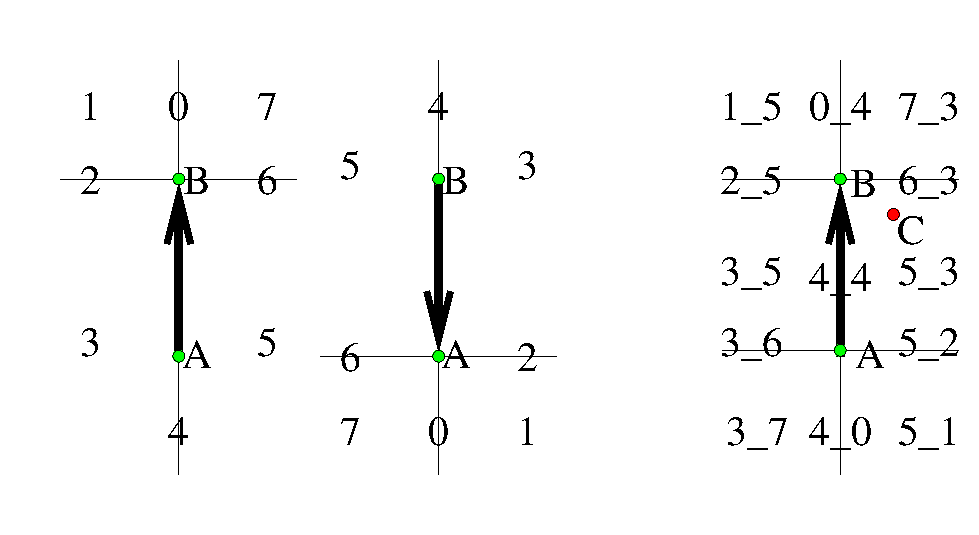
\includegraphics[height=4.3cm]{Doublecross_classic}
	\caption{The two Single Cross reference frames resulting in the overall Double Cross Calculus reference frame}
	\label{fig:DCC}
\end{figure}


\kasten{
\subsubsection*{Alternative Doublecross Calculus (DCC) overview}
\begin{calcfeatures}
\feature{calculus identifier}{adcc, alternative-double-cross}
\feature{calculus parameters}{none}
\feature{arity}{ternary}
\feature{entity type}{2D points}
\feature{description}{relates the referent $C$ relative to the line between origin $A$ and relatum $B$ and the orthogonal lines through $A$ and $B$, resulting in 17 base relations}
\feature{base relations}{0-12, a, b, dou, tri}
\lastfeature{references}{\citet{cosyfre92}}
\end{calcfeatures}
}

In the literature also a single numbered notation can be found.
We refer to this nomenclatur as the Alternative Doublecross Calculus.
Apart from relations $b\uline 4$, $4\uline a$ the mapping between tuple notation and alternative
notation is given in Figure \ref{fig:DCC_Table_alternative}.
$b\uline 4$ corresponds to \textbf{b} and $4\uline a$ to \textbf{a}.
\textbf{dou} and \textbf{tri} are defined as above.

\begin{figure}[h!]
	\centering
	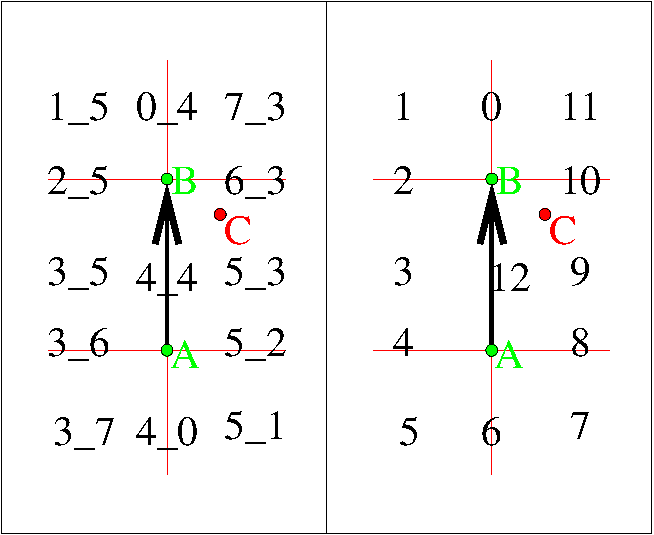
\includegraphics[height=4cm]{Doublecross_new}
	\caption{Schematic overview of Doublecross base relation names
	in tuple notation and the alternative notation.}
	\label{fig:DCC_Table_alternative}
\end{figure}

